\documentclass[]{report}
\usepackage{graphicx, float}
\usepackage[export]{adjustbox}

\title{\centering CSP334 : Computer Networks \\Lab Assignment No 3\\Assignment on traceroute, ping commands}
\author{\LARGE Sahil\\2016UCS0008}

% to use proper section numbering in the report type 
\renewcommand{\thesection}{\arabic{section}}

\begin{document}

\maketitle

%%%%%%%%%%%%%%%%%%%%%%%%%%%%%%%%%%%%%%%%%%%%%%%%
\section{Working of \textit{traceroute}:}
\textbf{Brief explanation of its working}: 
\\ 
It works by sending packets with TTL values starting from 1 onwards. The packet with TTL 1 reaches the first router, which then responds with ICMP TTL exceeded message, and at the source, its IP address is known from this response packet. Similarly, the packet with TTL 2 reaches the next router, and the process repeats till destination IP is reached or maximum limit of TTL packets has been sent and time out occurs. 

\subsection{If there were no TTL field in the invocation of the \textit{traceroute} at all:}
then we cannot identify the routers in between the source and destination, as the packet would return back only if it reaches the destination or if the TTL value becomes 1 at some point.

\subsection{Routers determine whether the TTL value limit has reached:} 
by decrementing the value of the TTL by $1$ as soon as it  reaches the router, so whenever a router gets a packet with a TTL value of $1$, it knows that the TTL value limit has been reached.

\subsection{Intermediate route receiving a packet with ICMP TTL exceeded message: }
should not respond again as it already contains TTL exceeded message sent by another router whose IP address should be made available to the source. 

\subsection{\textit{traceroute} makes use of destination UDP port number which is invalid} 
so that when it reaches the destination, the connection cannot be established and an error message is returned as the response. Morever, it helps in distinguishing that the destination has reached since previous responses would be ICMP TTL exceeded, so the INVALID UDP PORT message identifies that we have reached the destination.

\subsection{Address of all the routers in between us and destination}
is known as the command sends packets with different TTL values starting from 1 to some maximum value, so the one with value of 1 reaches the first router and then router responds with TTL exceeded message, so it sends along its IP address which is thus known at the source. Similarly, IPA of all the routers in between is known. 

\subsection{\textit{traceroute} latency}
is calculated in terms of the \textbf{round trip time}. When the packet is sent from source, a time stamp is put indicating the start time, so after reaching the router which sends a ICMP TTL exceeded message, when the message arrives at the source, the current time is noted, so the difference of the times is the RTT.

%%%%%%%%%%%%%%%%%%%%%%%%%%%%%%%%%%%%%%%%%%%%%%%%
\section{Problem 2:  Executing \textit{traceroute} command: }
\begin{figure}[H]
	\vspace{0pt}
	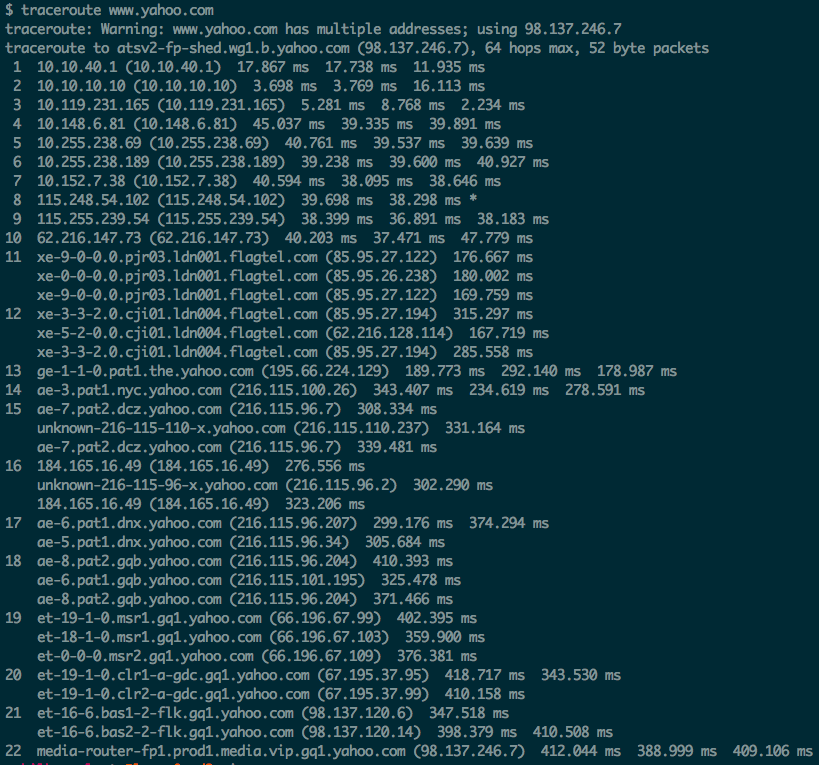
\includegraphics[height = 350pt, keepaspectratio]{Snapshots/exe2/exe2_2.png}
\end{figure}

\subsection{IPA of \textit{www.yahoo.com}}
The IPA obtained from traceroute is : \textbf{$98.137.246.7$}

\subsection{No. of iterations to determine the route is:} $22$

\subsection{IPA of all the machines between source and destination are: }
\begin{itemize}
	\item $10.10.40.1$
	\item $10.10.10.10$
	\item $10.119.231.165$
	\item $10.148.6.81$
	\item $10.255.238.69$
	\item $10.255.238.189$
	\item $10.152.7.38$
	\item $115.248.54.102$
	\item $115.255.239.54$
	\item $62.216.147.73$
	\item $85.95.27.122$
	\item $85.95.27.194$
	\item $195.66.224.129$
	\item $216.115.100.26$
	\item $216.115.96.7$
	\item $184.165.16.49$
	\item $216.115.96.207$
	\item $216.115.96.204$
	\item $66.196.67.99$
	\item $67.195.37.95$
	\item $98.137.120.6$
	\item $98.137.246.7$
\end{itemize}

\subsection{Avg. Round trip time of the packet that reached the destination is:}
$403.38$ milli seconds

%%%%%%%%%%%%%%%%%%%%%%%%%%%%%%%%%%%%%%%%%%%%%%%%
\section{Problem 3: \textit{traceroute} and \textit{tcpdump}}
\textit{\$ sudo tcpdump -n -v udp -c 10} command is run in one window and 
\\
 \textit{\$ traceroute www.yahoo.com} command is run then. The output is shown in the figure. 

\begin{figure}[H]
	\vspace{0pt}
	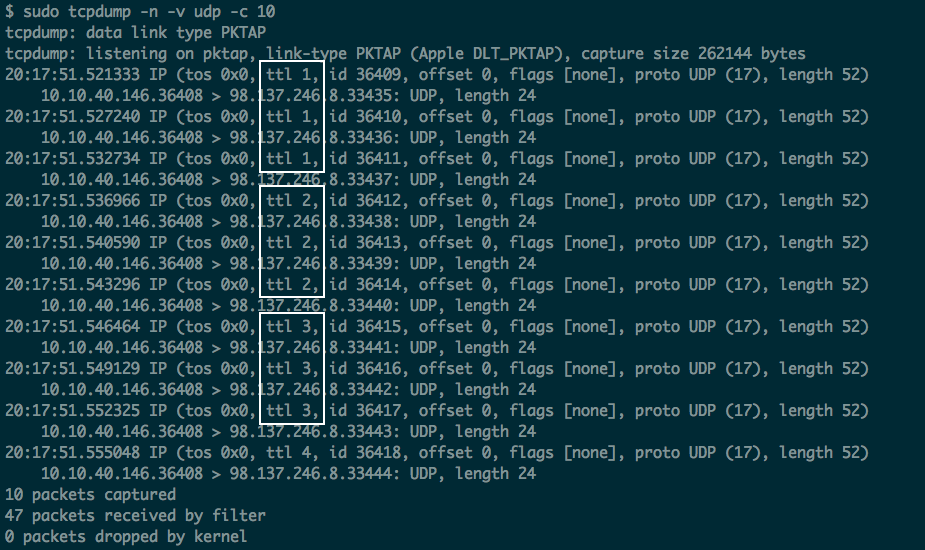
\includegraphics[height = 250pt, keepaspectratio]{Snapshots/exe3/q3_1.png}
\end{figure}

\subsection{Packets sent in one iteration:}
\textit{traceroute} sends $3$ packets in $1$ iteration. This is proved from the above figure, as highlighted, there are 3 packets for each TTL value starting from 1.

\begin{figure}[H]
	\vspace{0pt}
	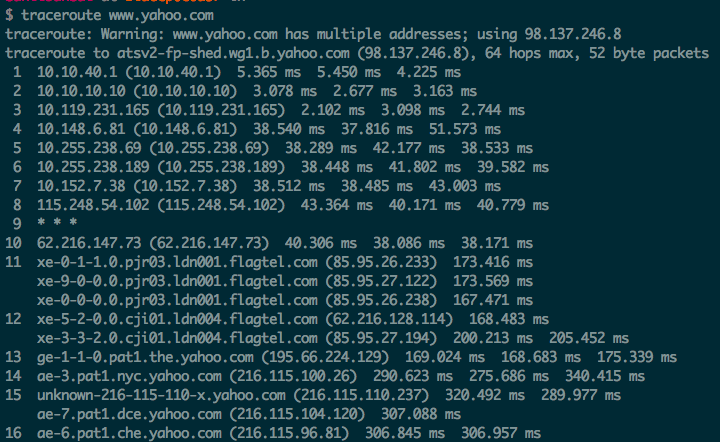
\includegraphics[height = 250pt, keepaspectratio]{Snapshots/exe3/q3_2.png}
\end{figure}

\subsection{Round trip time:}
For one specific iteration (consider $14^{th}$), individual RTT's of the three probes are: $290.623$ms, $275.686$ms, $340.415$ms. The avg. RTT is: $302.24$ms. Comparing it with the individual RTT's, there is a lot of deviation. This is because the RTT depends on the forward path as well as the reverse path, thus, there may be some delays in the reverse path in the 3rd packet, as its RTT is lot higher than the other 2. 

\subsection{Port numbers used:}
\begin{figure}[H]
	\vspace{0pt}
	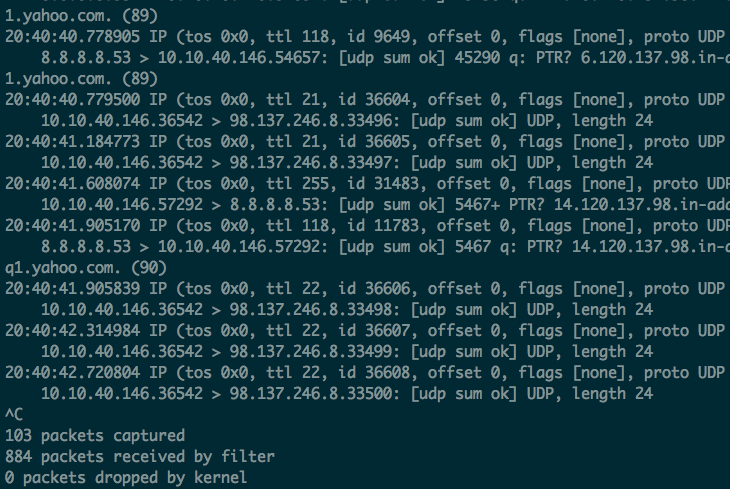
\includegraphics[height = 250pt, keepaspectratio]{Snapshots/exe3/q3_3.png}
\end{figure}

For each iteration, it uses different port numbers for the destination. As in the above figure, for TTL 21, port numbers used are: 33496, 33497 whereas for TTL 22, port numbers 33498,  33499, 33500 are used.  This might be because simultaneously packets might come to the destination at the same port otherwise. 

%%%%%%%%%%%%%%%%%%%%%%%%%%%%%%%%%%%%%%%%%%%%%%%%
\section{Problem 4: Visual \textit{traceroute}}
\begin{figure}[H]
	\vspace{0pt}
	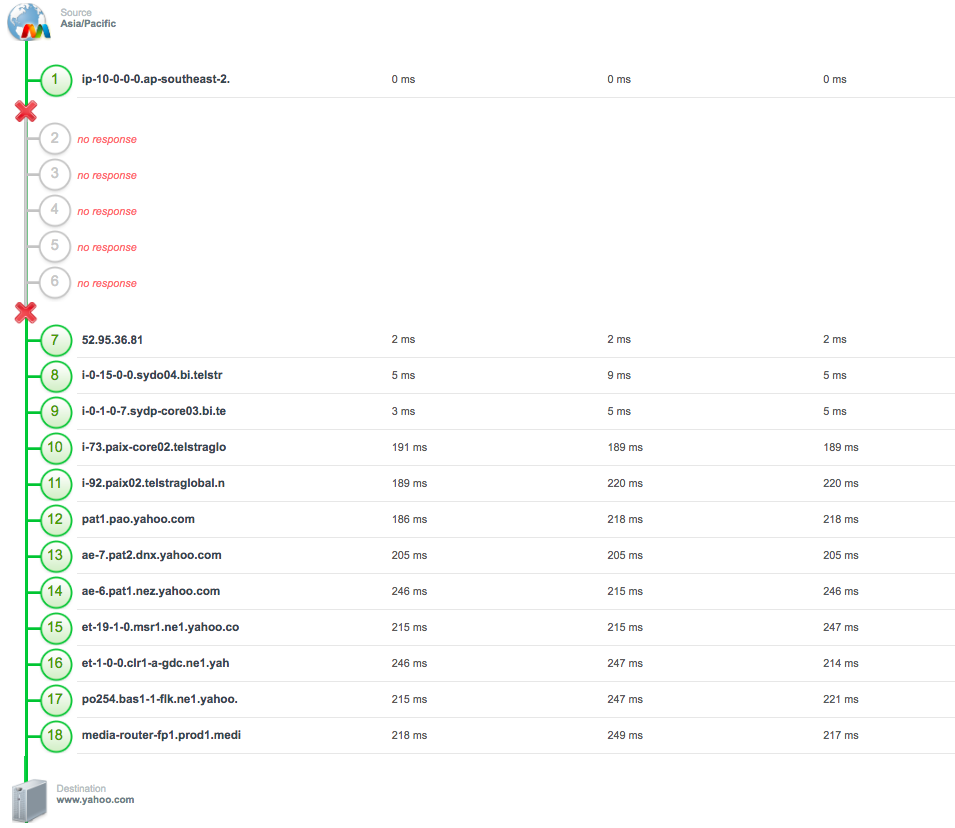
\includegraphics[height = 350pt, keepaspectratio]{Snapshots/exe4/q4_1.png}
\end{figure}

\begin{figure}[H]
	\vspace{0pt}
	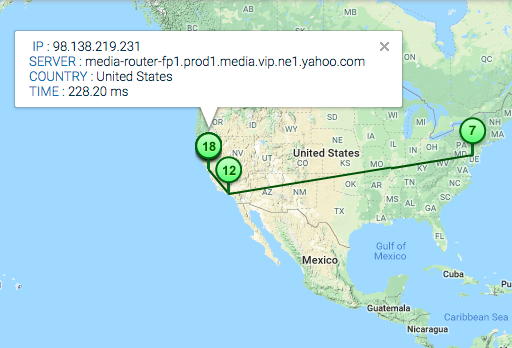
\includegraphics[height = 200pt, keepaspectratio]{Snapshots/exe4/q4_2.png}
\end{figure}

\begin{itemize}
	\item Source IP address: $52.95.36.81$
	\item Destination IP address: $98.138.219.231$
\end{itemize}
%%%%%%%%%%%%%%%%%%%%%%%%%%%%%%%%%%%%%%%%%%%%%%%%
\section{Problem 5: Knowing whether firewall has come in the way}
We can know that a firewall has come into way and stopped the packet, if we are unable to reach to the destination while using the traceroute command. As seen in the figure below, * * * starts appearing in the output.
\begin{figure}[H]
	\vspace{0pt}
	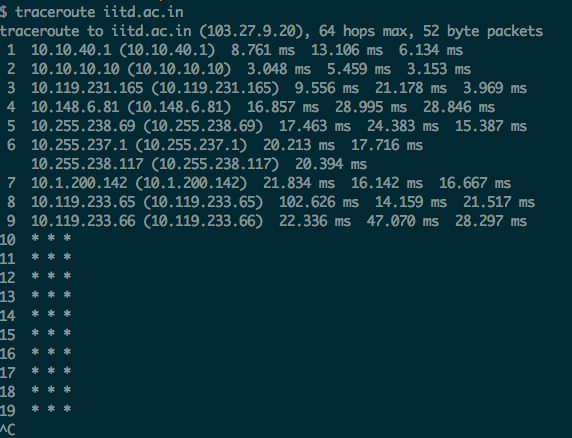
\includegraphics[height = 200pt, keepaspectratio]{Snapshots/exe5/q5_1.png}
\end{figure}

But, when the same \textit{traceroute} command is used with \textbf{-I} option, i.e. sending ICMP requests only, we get the complete output: 
\begin{figure}[H]
	\vspace{0pt}
	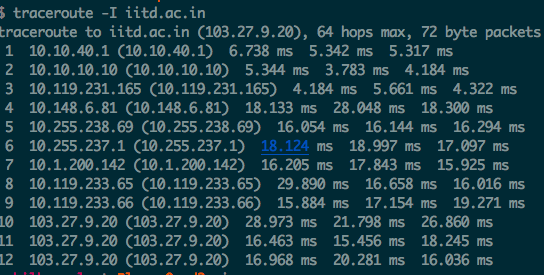
\includegraphics[height = 200pt, keepaspectratio]{Snapshots/exe5/q5_2.png}
\end{figure}
Thus, the IP address of the firewall is based on the destination IP address as the last few IP addresses are similar in the above output.

%%%%%%%%%%%%%%%%%%%%%%%%%%%%%%%%%%%%%%%%%%%%%%%%
\section{Problem 6: Last IP address in \textit{traceroute}}
If a firewall has not obstructured the packet sent, the last IP address appearing in the \textit{traceroute} must indicate the IP address of the destination as traceroute command terminates when it receives UDP Port INVALID response from the destination IP. In the above figure shown for problem 5, clearly the IPA of destination matches the last IPA.

%%%%%%%%%%%%%%%%%%%%%%%%%%%%%%%%%%%%%%%%%%%%%%%%
\section{Problem 7: Usages of the \textit{ping} program}
\begin{figure}[H]
	\vspace{0pt}
	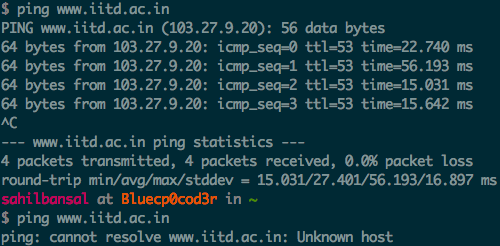
\includegraphics[height = 150pt, keepaspectratio]{Snapshots/exe7/q7_1.png}
\end{figure} 
\begin{itemize}
	\item Ping is mainly used to check whether a machine is connected to the network. It also displays the round trip times. As in the figure shown above, the second ping command is unable to resolve the host as the machine is not connected to the network.
	\begin{figure}[H]
		\vspace{0pt}
		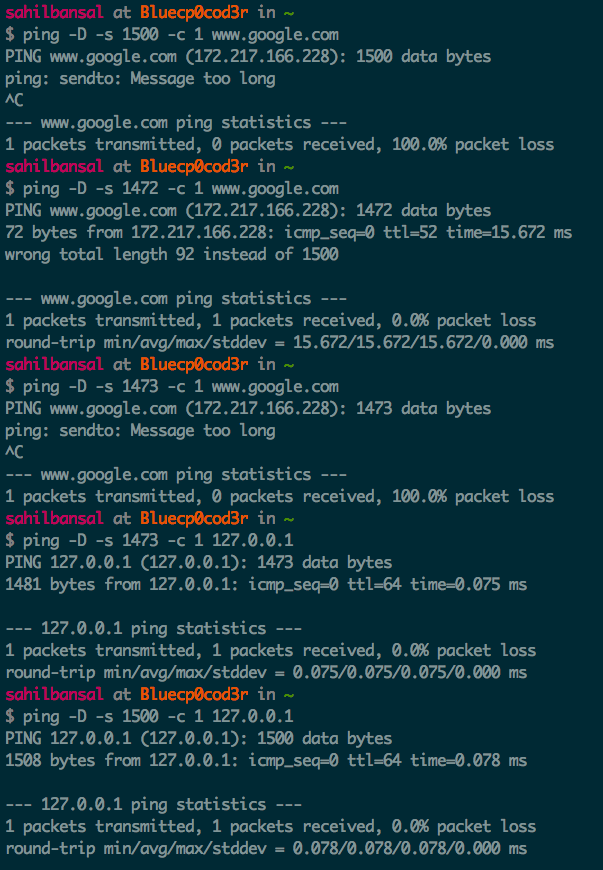
\includegraphics[height = 400pt, keepaspectratio]{Snapshots/exe7/q7_2.png}
	\end{figure} 
	\item It can be used to know the maximum frame size of message allowed by the Network Interface Card. As in the figure shown above, the \textbf{-D} option is used to set the \textbf{don't fragment} bit and \textbf{-s} option is used to specify the size of the packet, so we get the reply \textbf{Message too long}, if the size exceeds the maximum allowed message size. 
	\\
	We can see from the first 3 commands in above figure, that the maximum size allowed is 1472, this is because after adding the headers at the link layer (8 bytes) and network layer (28 bytes), the size becomes 1500 which is the default maximum allowed size. 
	\\
	Also, it allows sending any size packet to the localhost since it is the same machine, and also adds only 8 bytes of header (link layer), since there is no need of network layer in this case. 
	\item It can be used to identify the presence of a firewall as some good firewalls block time stamp requests and source routed packets. 
\end{itemize}
%%%%%%%%%%%%%%%%%%%%%%%%%%%%%%%%%%%%%%%%%%%%%%%%
\section{Problem 8: Using ping to simulate the working of \textit{traceroute}}
A file named \textbf{ping\_as\_traceroute} is created which contains the shell srcipt to use \textit{ping} as \textit{traceroute}. It is displayed below:
\begin{figure}[H]
	\vspace{0pt}
	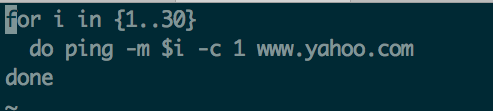
\includegraphics[height = 50pt, keepaspectratio]{Snapshots/exe8/q8_1.png}
\end{figure} 
The \textbf{-m} option is used to send packet with a specific TTL value, and -c option is used to send a particular no. of packets. So for all TTL values from $1$ to $30$, we send a single packet, and in response we get the IPA of all the routers in between the source (our machine) and the destination. This value $30$ can be large if we reach the destination in first few iterations only, so it is just a maximum value chosen for convenience, we can adjust it by hit and trial.
\\
The ouptut received is displayed in the following figure:
\begin{figure}[H]
	\vspace{0pt}
	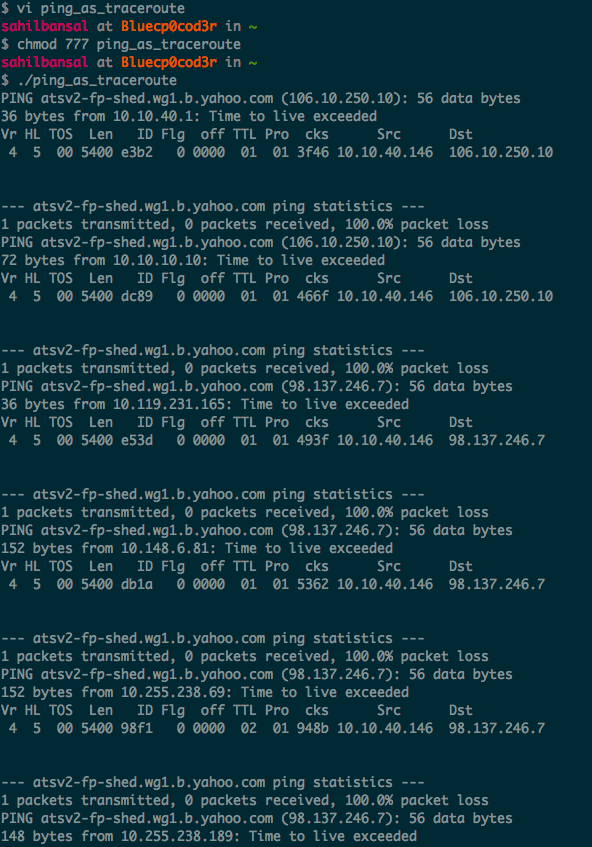
\includegraphics[height = 400pt, keepaspectratio]{Snapshots/exe8/q8_2.png}
\end{figure} 

%%%%%%%%%%%%%%%%%%%%%%%%%%%%%%%%%%%%%%%%%%%%%%%%
\section{Problem 9: Approaches that can be used to do a \textit{ping sweep}}
Ping sweep is used to find which range of IP addresses are active on a host. It sends multiple ICMP requests to multiple hosts. If the given address is live, the response is received. The various methods to do ping sweep are:
\begin{itemize}
  	\item \textbf{nmap:}
	nmap is a tool for generally used for port scanning. The \textbf{-sP} option can be used with it to do ping sweeping. The range of IPA can then be specified. It then works similar to ping my sending ICMP requests and waiting for a response before sending the next packet to the next host. 
	\begin{figure}[H]
		\vspace{0pt}
		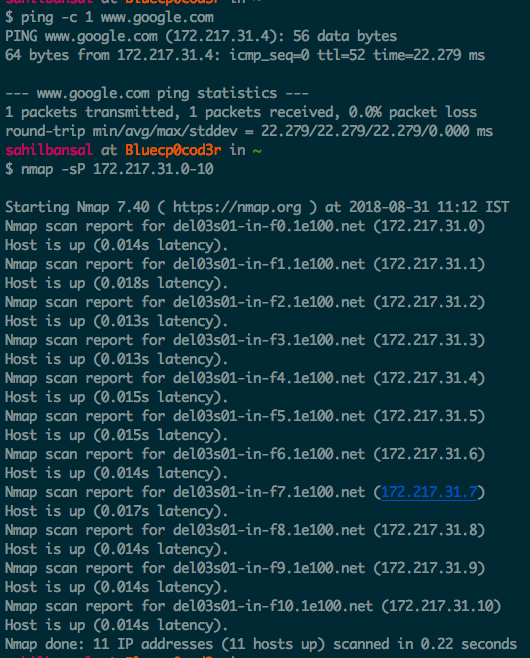
\includegraphics[height = 300pt, keepaspectratio]{Snapshots/exe9/q9_1.png}
	\end{figure}
	\item \textbf{fping:}
	It works a little differently than ping sending multiple ICMP requests at the same time and not waiting for the respons before sending the next one. As seen in the output below the result for $172.217.167.1$ is arrived before $172.217.167.0$. This proves it. The \textbf{-g} option is used to specify the start and the end IPA for the ping sweep. 
	\begin{figure}[H]
		\vspace{0pt}
		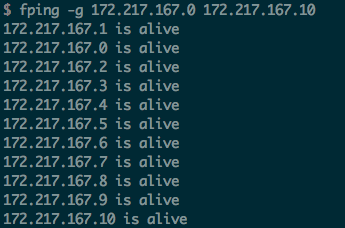
\includegraphics[height = 150pt, keepaspectratio]{Snapshots/exe9/q9_3.png}
	\end{figure}  
	\item \textbf{nmap using TCP:}
	nmap can also be used to do ping sweep by sending TCP requests instead of ICMP requests. The \textbf{-PT} option can be used followed by the port number without any space to specify the port number on which to send the request. As seen in the below output, the host is alive only when sending a request on port 80 since that is the standard HTTP port and we are doing ping on google, so it doesn't respond on other ports. 
	\begin{figure}[H]
		\vspace{0pt}
		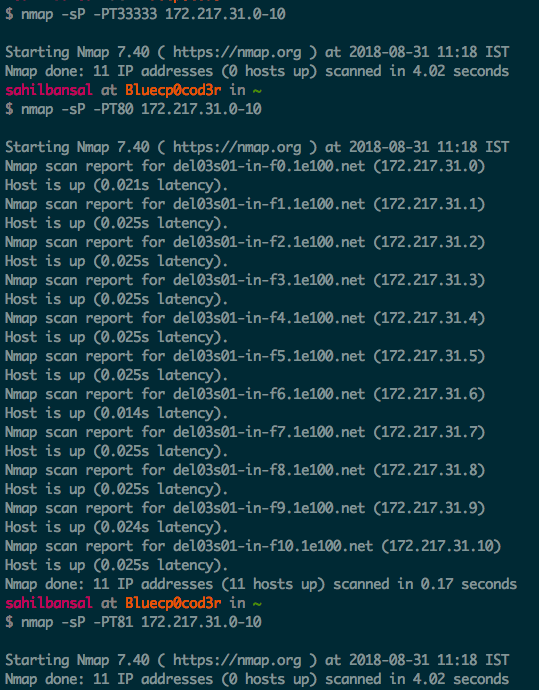
\includegraphics[height = 300pt, keepaspectratio]{Snapshots/exe9/q9_2.png}
	\end{figure}  
	\item \textbf{bash for loop:}
	We can write a for loop for doing a ping sweep by running ping to different address each time. As in the below output, we ping all IP addresses from $172.217.167.0 - 172.217.167.10$. 
	\begin{figure}[H]
		\vspace{0pt}
		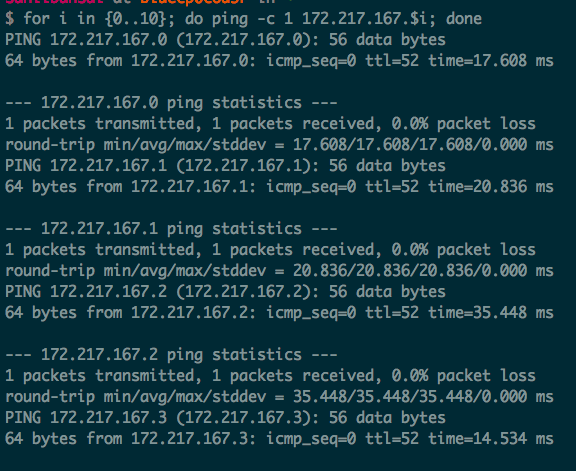
\includegraphics[height = 200pt, keepaspectratio]{Snapshots/exe9/q9_4.png}
	\end{figure}  
\end{itemize}
\end{document}